\begin{frame}
    \frametitle{Научная новизна}
    \begin{itemize}
  \item {Выявлены закономерности переноса знаний при псевдоразметке данных для многозадачных нейросетевых моделей с одним линейным слоем.}
  \item {Выявлены закономерности переноса знаний в энкодер-агностичных многозадачных нейросетевых моделях между различными диалоговыми задачами и языками. Была получена оценка зависимости этого переноса от размера обучающей выборки. Была проверена также справедливость выводов о межъязыковом переносе для однозадачных моделей.}
  \item {Получена оценка зависимости межъязыкового переноса знаний на разговорных данных в многоязычных нейросетевых моделях от размера предобучающей выборки и генеалогической близости языков к языку дообучения.}
  \item {Разработана диалоговая платформа DREAM и показана ее пригодность для изучения прикладного применения многозадачных нейросетевых моделей.}
  \item {Рассмотренные в диссертации многозадачные нейросетевые архитектуры были интегрированы в диалоговую платформу DREAM, была оценена их применимость и был проведен их сравнительный анализ на основе опыта применения. На основании этого анализа была произведена также интеграция в библиотеку DeepPavlov, находящуюся в открытом доступе.}
    \end{itemize}
\end{frame}
\note{
}

\begin{frame}
    \frametitle{Практическая значимость}
    \begin{itemize}
   \item Впервые в России была создана диалоговая платформа мирового уровня, вышедшая в полуфинал престижных мировых конкурсов Alexa Prize 3 и Alexa Prize 4 (в конкурсах было 10 и 9 участников соответственно, из более чем 300 кандидатов). Эта диалоговая платформа имеет полностью открытый код, что дает возможность легкого переиспользования любой части проделанной над ней работы. Были также разработаны сценарные навыки для этой платформы.
   \item В данной диалоговой платформе были применены многозадачные нейросетевые модели: многозадачная нейросетевая модель с одним линейным слоем, многозадачная нейросетевая модель на основе архитектуры PAL-BERT и многозадачная энкодер-агностичная нейросетевая модель.
   \item Программный код для реализации многозадачной энкодер-агностичной нейросетевой модели встроен в библиотеку DeepPavlov, имеющую более 500000 скачиваний на март 2023 года.
    \end{itemize}
\end{frame}
\note{
}


\iffalse
\begin{frame}
    \frametitle{Акт о внедрении}
    \begin{figure}[h]
        \centering
        \fbox{
            \begin{minipage}[t]{0.4\linewidth}
                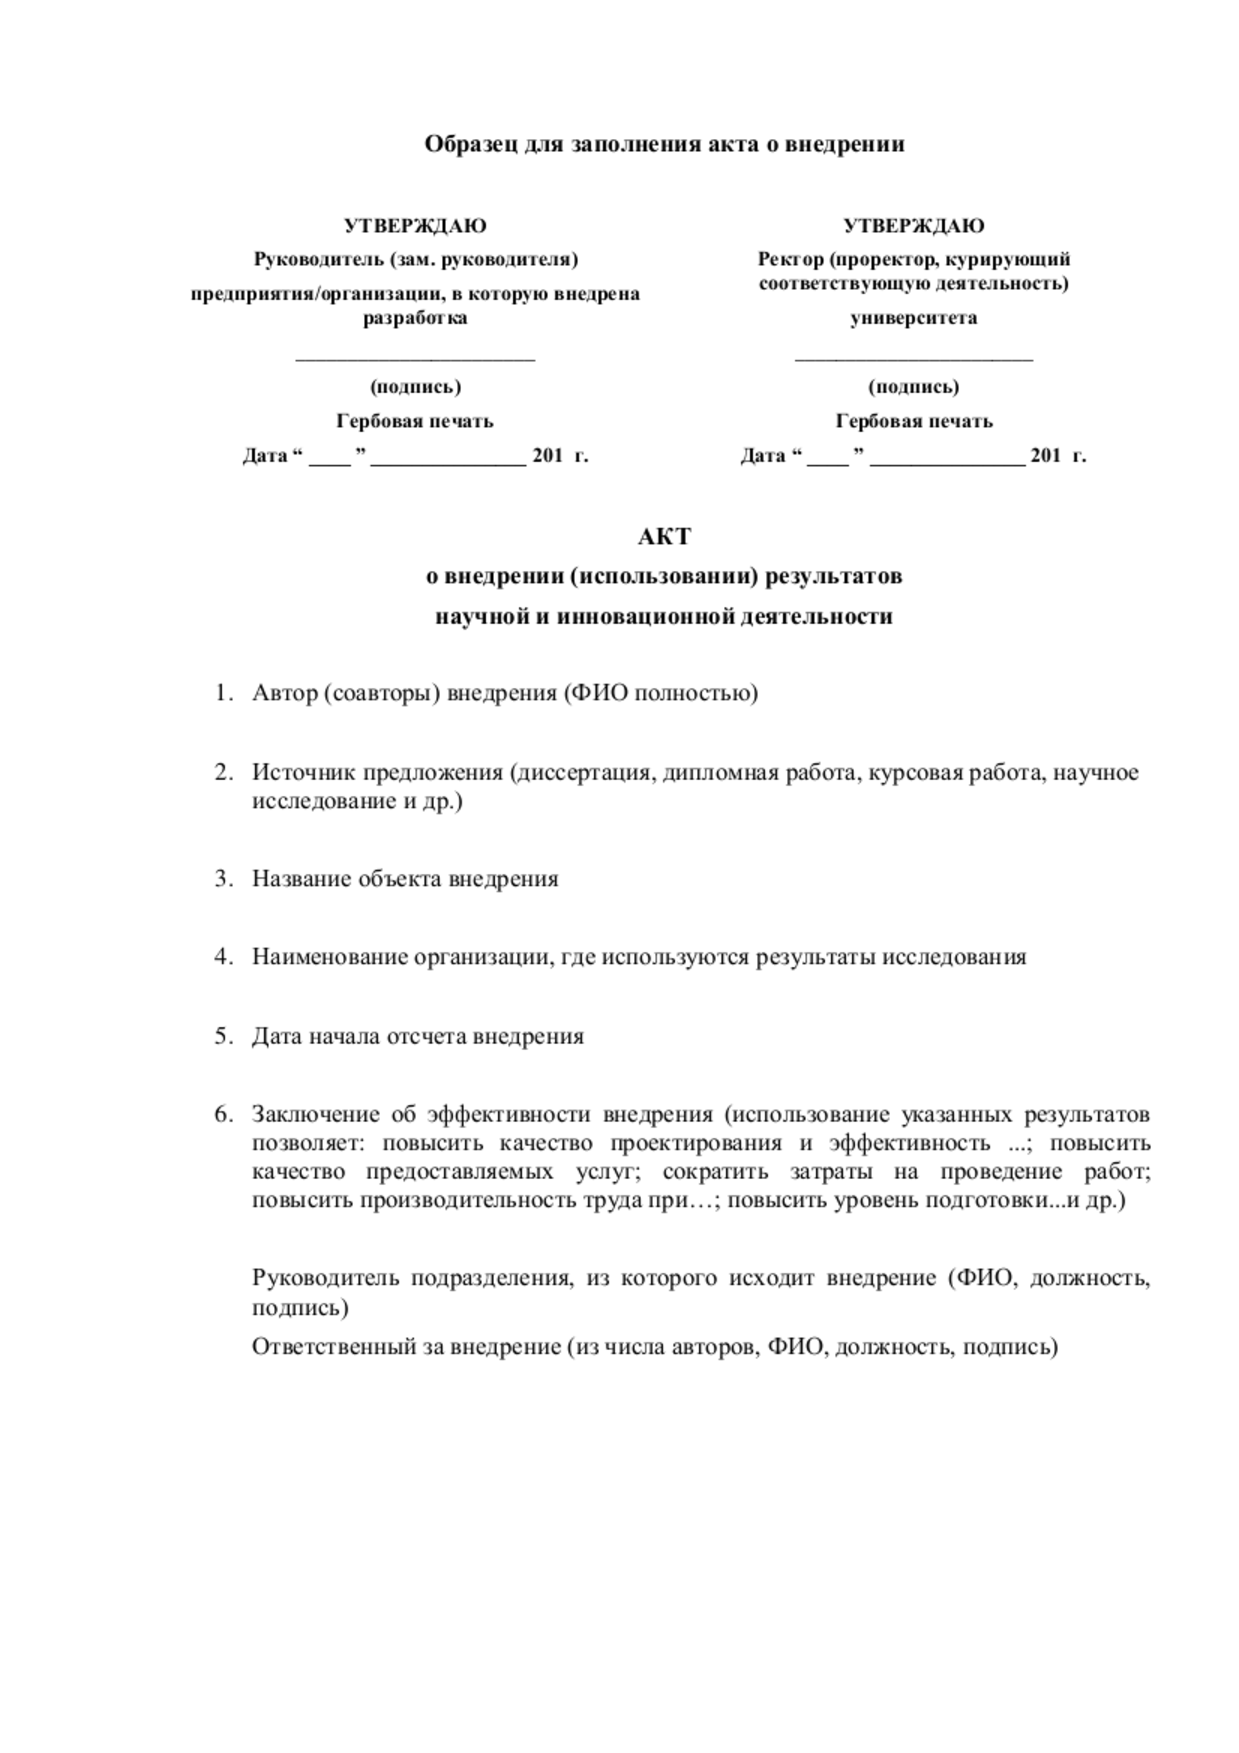
\includegraphics[width=\linewidth]{implementation}
            \end{minipage}
        }
    \end{figure}
\end{frame}
\note{
    Получен акт о внедрении.
}
\fi

% \begin{frame} % публикации на одной странице
\begin{frame}[t,allowframebreaks] % публикации на нескольких страницах
    \frametitle{Основные публикации}
    \nocite{pseudolabel}
    \nocite{rumtl}%
    %\nocite{enmtl}%
    \nocite{rutopics}
    \nocite{dream1}
    \nocite{dream1_trudy}
    \nocite{dream2}
    \nocite{dp_2023}
    \ifnumequal{\value{bibliosel}}{0}{
        \insertbiblioauthor
    }{
        \printbibliography%
    }
\end{frame}
\note{
    Результаты работы опубликованы в N печатных изданиях, в т.ч. M реферируемых изданиях.
}

\begin{frame}
    \frametitle{О результатах доложено на конференциях}
    \begin{itemize}
   \item En\&T 2018, доклад «Разработка диалоговой системы с интеграцией профиля личности», Даниил Болотин, Дмитрий Карпов, Григорий Рашков, Иван Шкурак, 15-16 ноября 2018 года, Москва;
   \item Диалог-2021, доклад «Data pseudo-labeling while adapting BERT for multitask approaches», Dmitry Karpov, Mikhail Burtsev, 16-19 июня 2021 года, Москва;
   \item AINL-2023, доклад «YAQTopics: Russian Conversational Topic Dataset», Dmitry Karpov, Vasily Konovalov, Mikhail Burtsev, 20-22 апреля 2023 года, Ереван, Армения
    \end{itemize}
\end{frame}
\note{
}

\begin{frame}[plain, noframenumbering] % последний слайд без оформления
    \begin{center}
        \Huge
        Спасибо за внимание!
    \end{center}
\end{frame}
